\documentclass[a4paper, 12pt, english]{article}

% \usepackage[portuges]{babel}
\usepackage[utf8]{inputenc}
\usepackage{amsmath,amssymb}
\usepackage{graphicx}
\usepackage{subfig}
\usepackage[colorinlistoftodos]{todonotes}

\usepackage{indentfirst}
\usepackage{verbatim}
\usepackage{textcomp}
\usepackage{gensymb}
\usepackage{float}

\usepackage{relsize}

\usepackage{lipsum}% http://ctan.org/pkg/lipsum
\usepackage{xcolor}% http://ctan.org/pkg/xcolor
\usepackage{xparse}% http://ctan.org/pkg/xparse
\NewDocumentCommand{\myrule}{O{1pt} O{2pt} O{black}}{%
	\par\nobreak % don't break a page here
	\kern\the\prevdepth % don't take into account the depth of the preceding line
	\kern#2 % space before the rule
	{\color{#3}\hrule height #1 width\hsize} % the rule
	\kern#2 % space after the rule
	\nointerlineskip % no additional space after the rule
}
\usepackage[section]{placeins}

\usepackage{booktabs}
\usepackage{colortbl}%
\newcommand{\myrowcolour}{\rowcolor[gray]{0.925}}

\usepackage[obeyspaces]{url}
\usepackage{etoolbox}
\usepackage[colorlinks,citecolor=black,urlcolor=blue,bookmarks=false,hypertexnames=true]{hyperref}

\usepackage{geometry}
\geometry{
	paper=a4paper, % Change to letterpaper for US letter
	inner=3cm, % Inner margin
	outer=3cm, % Outer margin
	bindingoffset=.5cm, % Binding offset
	top=2cm, % Top margin
	bottom=2cm, % Bottom margin
	%showframe, % Uncomment to show how the type block is set on the page
}
\usepackage{fancyhdr}

% Define header and footer
\pagestyle{fancy}
\fancyhf{}
\lhead{ENER 104L}
\rhead{iSciM, Habib University} % Right-aligned page number in the header
\rfoot{\thepage} % Right footer text
%*******************************************************************************%
%************************************START**************************************%
%*******************************************************************************%
\begin{document}

%************************************TITLE PAGE**************************************%
\begin{titlepage}
	\begin{center}
		\textbf{\LARGE Habib University}\\[0.5cm]
		\textbf{\large iSciM}\\[0.2cm]
		\textbf {\large Fall 2023}\\[0.2cm]
		\vspace{20pt}
		
\includegraphics[width=5cm]{../habiblogo.jpg}\\[1cm]
		\par
		\vspace{20pt}
		\textbf{\Large ENER 104L RENEWABLE ENERGY}\\
		\vspace{15pt}
		\myrule[1pt][7pt]
		\textbf{\LARGE  LABORATORY REPORT 6}\\
		\vspace{15pt}
		\textbf{\large Biodiesel}\\
		\myrule[1pt][7pt]
		\vspace{25pt}
		\begin{tabular}{@{}p{5cm}p{3cm}@{}}
			\textbf{\large Student Name} & \textbf{\large Student ID} \\
			Ali Asghar Yousuf            & ay06993                    \\ % No1 
			Syed Ibrahim Ali Haider      & sh06565                    \\ % No2
		\end{tabular}

		\vspace{10pt}
		\begin{tabular}{@{}p{5cm}p{3cm}@{}}
			\textbf{\large Group Name} & \textbf{\large Group No.} \\
			Insane Fr                  & 1                         \\
		\end{tabular}

		\vspace{45pt}
		\textbf {\large Lab Instructors:}\\[0.2cm]
		\Large {Paishwa Naqvi}\\[0.1cm]
		\Large {Amber Talat}\\[0.1cm]
		\Large {Mah Noor Jamil}\\[0.1cm]
	\end{center}

	\par
	\vfill
	\begin{center}
		\textbf{\today}\\
	\end{center}

\end{titlepage}

%************************************TABLE OF CONTENTS**************************************%

%  %Sumário
%  \newpage
%  \tableofcontents
%  \thispagestyle{empty}
%  %End Sumário

%********************************%
%***********SECTION 1************%
%********************************%
\newpage
\section{Objectives}
\begin{itemize}
	\item Create Biodiesel using vegetable oil, methanol and potassium hydroxide
	\item Perform the 3/27 test to confirm if full conversion from vegetable oil to
	      biodiesel was achieved
\end{itemize}

\section{Abstract}
Biodiesel is a renewable fuel that can be used in diesel engines. It is made
from vegetable oil, methanol and a catalyst. In this experiment, we made
biodiesel by mixing vegetable oil, methanol and potassium hydroxide at
$50-55\degree C$. We then tested the biodiesel produced using the 3/27 test.
The 3/27 test is done by mixing 3 ml of biodiesel with 27 ml of methanol at
$20-22\degree C$. The mixture is then observed for any signs of fall out. If
there is no fall out, then the reaction went well and we achieved full
conversion.

\section{Result and Analysis}
\subsection{Creating Biodiesel}
We created biodiesel by mixing 150 ml of vegetable oil, with 30 ml of methanol
with 1 gram of potassium hydroxide dissolved in it.

\begin{table}[H]
	\centering
	\begin{tabular}{|l|p{5cm}|l|p{5cm}|}
		\toprule
		\textbf{Temperature} & \textbf{Input}                                                    & \textbf{Color} & \textbf{Observation}                                                    \\ \midrule
		23                   & Vegetable oil put on heat with stirrer                            & Yellow         & No change                                                               \\ \bottomrule
		30                   & No input                                                          & Yellow         & Bubbles forming                                                         \\ \bottomrule
		40                   & No input                                                          & Yellow         & Bubbles intensifying                                                    \\ \bottomrule
		50                   & Heat and stirrer turned off and Methanol with dissolved KOH added & Light brown    & Two layers starting to form                                             \\ \bottomrule
		55                   & Stirrer turned on                                                 & Dark brown     & Some reaction taking place causing the mixture to heat up               \\ \bottomrule
		60                   & Stirrer turned off                                                & Dark brown     & Two layers formed, dark brown at the bottom and milky yellow at the top \\ \bottomrule

	\end{tabular}
	\caption{Observations during the biodiesel creation process}
\end{table}

\begin{figure}[H]
	\centering
	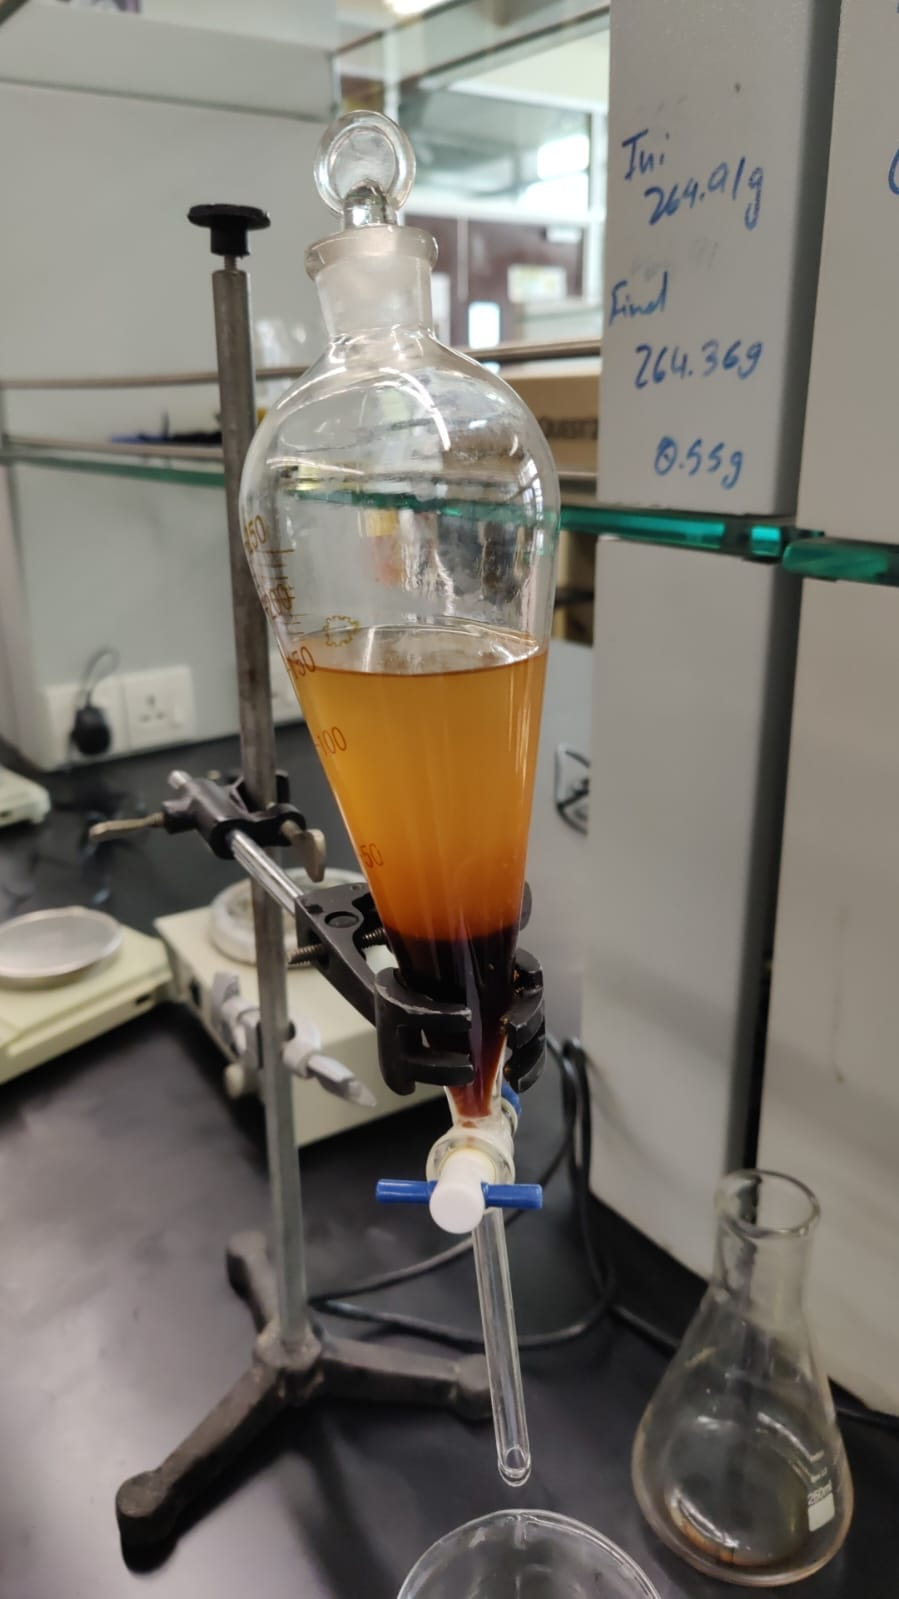
\includegraphics[width=0.5\textwidth]{images/biodiesel.jpg}
	\caption{Biodiesel and Glycerol}
\end{figure}

The reaction produces two products, biodiesel and glycerol. The biodiesel is
the yellow liquid at the top and the glycerol is the dark brown liquid at the
bottom. The glycerol is a byproduct of the transesterification reaction. The
biodiesel was then separated from the glycerol using a separatory funnel.

\subsection{3/27 Test}
The 3/27 test was performed by mixing 3 ml of biodiesel with 27 ml of methanol
at $20-22\degree C$. The mixture was then set aside for 10 minutes and observed
for any signs of fall out or separation by tilting the bottle and observing the
mixture. We observed no signs of fall out or separation. This means that the
reaction went well and we achieved full conversion.

\section{Conclusion}
We successfully created biodiesel using vegetable oil, methanol and potassium
hydroxide. We then performed the 3/27 test to confirm that we achieved full
conversion. We observed no signs of fall out or separation. This means that the
reaction went well and we achieved full conversion. The biodiesel produced can
be used in diesel engines. It is a renewable fuel and is better for the
environment than fossil fuels.

\section{Questions}
\begin{enumerate}
	\item Name the reactant used in production of biodiesel?

	      Vegetable oil, methanol and potassium hydroxide are used in the production of
	      biodiesel.

	\item Do you suggest any other feedstock to be used in laboratory as reactant?

	      We suggest using waste cooking oil as a feedstock. It is easily available and
	      is a waste product. It can be used to make biodiesel instead of being thrown
	      away.

	\item Does heating help to complete the process, if so, explain?

	      Heating helps to complete the process. It increases the rate of reaction. This
	      means that the reaction will be completed faster. It also helps to increase the
	      yield of the reaction. This means that the reaction will be more efficient\dots

	\item What ratio of the reactants is required to allow the reaction to proceed to
	      completion?

	      We used a ratio of 5:1 of vegetable oil to methanol. This allowed the reaction
	      to proceed to completion with full conversion.

	\item If you change the ratio of reactant, does it effect on product, why?

	      Changing the ratio of reactants will affect the product. If there is too much
	      methanol, then the reaction will not proceed to completion. If there is too
	      little methanol, then the reaction will proceed to completion but the yield
	      will be low. This means that the reaction will not be efficient and will
	      produce less biodiesel.

	\item What benefits do you think using biodiesel has compared to using traditional
	      diesel fuel?

	      Biodiesel is a renewable fuel. It is made from vegetable oil which is a
	      renewable resource. It is better for the environment than fossil fuels. It
	      produces less emissions and is biodegradable. It can be used in diesel engines
	      without any modifications. It is also safer to handle than fossil fuels.

	\item List four advantages of using biodiesel as a fuel.

	      \begin{enumerate}
		      \item Biodiesel is a renewable fuel.
		      \item Biodiesel is better for the environment than fossil fuels.
		      \item Biodiesel produces less emissions than fossil fuels.
		      \item Biodiesel is biodegradable.
	      \end{enumerate}

	\item Suggest and give details of any other biodiesel test.

	      Soap test can be used to test biodiesel. In this test, a sample of biodiesel is
	      mixed with water and shaken. If the biodiesel is pure, then it will not form
	      any bubbles. If the biodiesel is impure, then it will form bubbles. This is
	      because impure biodiesel contains soap which will react with water to form
	      bubbles.

	\item One argument against biodiesel being a “green” fuel is that combustion produces
	      $CO_2$, which is a greenhouse gas. Is it possible to counter this argument from
	      the standpoint of using renewable resources?

	      Yes, it is possible to counter this argument. The $CO_2$ produced by burning
	      biodiesel is absorbed by the plants used to make the biodiesel. This means that
	      the $CO_2$ is removed from the atmosphere. This makes biodiesel a carbon
	      neutral fuel.

\end{enumerate}

\end{document}